%------------------------------------------------------------------------------------
%	CHAPTER 1
%------------------------------------------------------------------------------------
\chapterimage{headMontagem.png}
\chapter{Entendimento Geral}

\begin{remark}
Machine Learning é a habilidade de localizar padrões em Dados. (Gil Weinberg - Founding Director of Georgia Tech Center for Music Technology) 
\end{remark}

\section{Do que trata esse livro?}\index{Entendimento Geral}
Cada vez que leio um livro de \textbf{Machine Learning} tenho a sensação que o autor quer mostrar para seus leitores o quanto ele é um bom Matemático, coloca um monte de fórmulas com demonstrações (muitas delas parecem escritas em grego e usam inclusive letras gregas) é isso me faz pensar: \textit{Será que quando indicar um livro para meus alunos vou querer que eles aprendam fórmulas ou que tenham uma base em que possam praticar?} 

E graças a isso publiquei uma série de artigos sobre os mais variados modelos de \textit{Machine Learning} na rede \textbf{Linkedin} e esses artigos foram a base para esse livro, não espere encontrar aqui muitos conceitos, apesar de ser obrigado a abordá-los ou muita coisa se perderia, mas a ideia aqui é ser totalmente prático.

Já ouvimos isso de prático tantas vezes, existe duas séries de livros especialistas denominadas: "\textit{Hands On}" e "\textit{Cookbook}". Aprecio e tenho muitos desses livros, porém sempre que desejo algo no primeiro caso é muito difícil encontrar bem separado e exposto da forma como queria e no segundo está fragmentado demais. O prático aqui será: Um modelo em linguagem Python, ler bases de dados, com o uso de suas possibilidades, seu treino e melhor forma de obter resultados. Sendo assim não espere encontrar nesse aulas básicas de Python.

\section{O que é Mineração de Dados?}\index{Entendimento Geral}
Antes de surgir o termo "Ciência de Dados", um artigo de 1996 chamado “\textit{Data Mining to knowledge discovery in database}” se referia a um processo geral de descoberta com a utilização das informações contidas nos dados. Em 2001, \textit{William S.Cleveland} levou a Mineração de Dados combinou esta com Ciência da Computação. Realizou estatísticas para expandir as possibilidades da Mineração de Dados.

Durante este período, surgiu a \textbf{Web 2.0} no qual sites não eram apenas um "Panfleto Digital", mas um meio para compartilhar, postar e comentar experiências entre milhões de usuários. Sites como \textit{Facebook} e \textit{Linkedin} (2003), \textit{Flickr} (2004), \textit{YouTube} e \textit{reddit} (2005), \textit{Twitter} e \textit{Spotify} (2006) ou \textit{Pinterest} (2010) que trouxeram muitos dados e se tornou difícil lidar com essa quantidade produzida. Assim criamos um novo termo denominado \textbf{Big Data}. Abriu um mundo de possibilidades para encontrarmos valores associados aos dados. Porém precisamos de infraestrutura para lidar com tantos dados, tecnologia de computação paralela como \textit{MapReduce}, \textit{Hadoop} e \textit{Spark}. Em 2010 ocorreu o surgimento da \textbf{Ciência de Dados} para dar suporte as necessidades de negócio.

\section{O que é Machine Learning?}\index{Entendimento Geral}
De forma bastante genérica, algorítimos de \textit{Machine Learning} (Aprendizado de Máquina e doravante apenas \textbf{ML}) são uma mudança de paradigma da “programação tradicional” onde precisamos passar toda a heurística explicitamente para um novo conceito, onde ao invés de escrever cada ação que o algorítimos deve realizar, apenas passamos diversos exemplos e deixamos que o computador resolva (ou aprenda) quais são as “melhores” (menor custo) decisões. É também chamada de \textit{Statistical Learning} (Autores Hastie, Tibshirani \& Friedman 2009) utilizada para extrair um modelo a partir de um sistema de observações ou medidas. Sendo um campo relativamente novo da ciência composto de uma variedade de métodos (algoritmos) computacionais e estatísticos que competem entre si.
\begin{figure}[H]
	\centering
	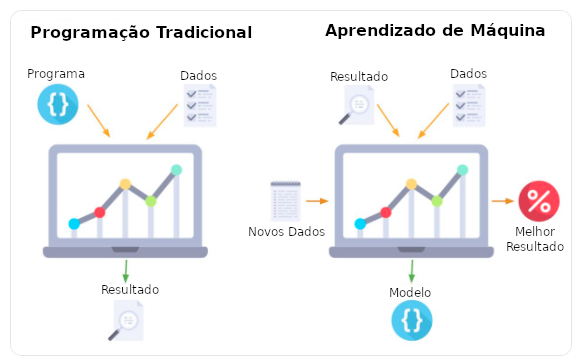
\includegraphics[width=0.65\textwidth]{cap01/EstruturaML.png}
	\caption{Programação Tradicional X Machine Learning}
\end{figure}

Ou seja, treinamos e melhoramos as respostas até que possam receber \textbf{novas observações}, transformamos isso em resultados sem que sejam explicitamente programáveis, isso é chamado "Modelo de ML". Interpretar esses modelos é entender como podemos transformar dados em informação útil. Em geral são classificados em:
\begin{itemize}[noitemsep]
	\item \textbf{Clusterização}: Encontrar uma estrutura de dados, sumarização.
	\item \textbf{Regressão e Estimação}: Predição de valores contínuos.
	\item \textbf{Classificação}: Predição de um item de um caso de classe/categoria.
	\item \textbf{Associação}: frequentemente ocorre entre itens e eventos.
\end{itemize}

É muito importante conhecer vários deles e assim podemos decidir qual se ajusta melhor as observações que temos para treiná-los. Devemos ter em mente que ML pode ser bem diferente de \textbf{Estatística}. Aqui não estamos preocupados com inferência, causalidade e exogeneidade. ML está mais preocupada, quase que exclusivamente, em melhorar predições ou rapidamente localizar em um mar de informações a resposta de um problema. 

Assim podemos pegar a mesma função, por exemplo \textbf{Regressão Logística} e analisar do ponto de vista da estatística, que interpretaria se os "betas" são significativos, se os "resíduos" têm uma distribuição normal ou analisar isso do ponto de vista de ML e descobrir como está a relação entre \textbf{Precisão} e \textbf{Recall}, ou qual a ROC ou AUC do modelo\footnote{As curvas ROC e AUC estão entre as métricas mais utilizadas para avaliação em um modelo de ML.}.

\section{Formas de Aprendizado}\index{Entendimento Geral}
Quanto as formas de aprendizado se dividem em:
\begin{itemize}[noitemsep]
	\item \textbf{Não Supervisionado}, corresponde a um vetor de observações que é utilizado para observar padrões, tendências, verificar estruturas e descobrir relações.
	\item \textbf{Supervisionado}, além do vetor de observações, existe também uma resposta associada a cada questão.
	\item \textbf{Aprendizagem por Reforço}, uma ação ocorre e as consequências são observadas, assim a próxima ação considera os resultados da primeira ação. É um algoritmo dinâmico que parte do princípio "tentativa e erro".
\end{itemize}

Entender a diferença entre os dois tipos é bem simples, enviamos ao computador uma série de imagens sobre pratos de comida e não informamos absolutamente nada sobre elas, o máximo que acontecerá é a separação dessas em grupos similares. Imaginemos que em seguida mostramos a seguinte imagem:
\begin{figure}[H]
	\centering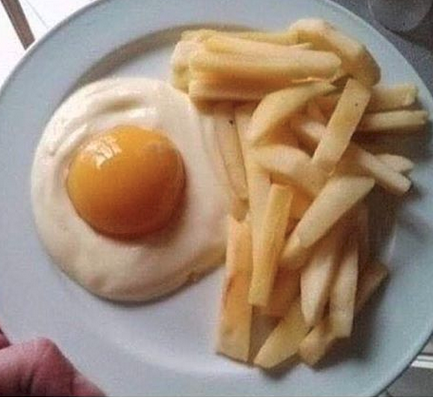
\includegraphics[scale=0.4]{cap01/visao.png}
	\caption{Nova informação}
\end{figure}

Qual será o prato de comida que o computador associará? Exatamente "Ovo frito e batatas fritas"\footnote{Apesar que se olhar mais de perto vemos que isso é iogurte, meio pêssego e tiras de maçã}. No segundo tipo de aprendizado além das imagens dizemos o que cada uma vem a ser, porém ao mostrar o mesmo tipo de imagem não pense que o computador consegue classificá-la corretamente, provavelmente pode se confundir mais uma vez (assim como nos confundimos com a imagem mostrada).

A resolução com problemas de imagem é bem complicada\footnote{Assim como análise da linguagem, chamada de NLP - \textit{Natural Language Processing}}, pois conseguimos identificar a diferença devido a nossa experiência não apenas visual mas com informações sobre textura, forma e outras que o computador ainda está engatinhando. Por isso o estudo desses algorítimos é algo tão rico e como vimos anteriormente. É muito importante conhecer boa parte dos modelos e decidir qual trabalha melhor com as observações que temos para treiná-lo.

\subsection{Algoritmo Não Supervisionado}
Não envolve um controle direto, aqui o ponto principal do requisito são desconhecidos e ainda precisam ser definidos. Normalmente são usados para: explorar uma estrutura de informação; extrair informações desconhecidas sobre as observações e detectar padrões.
\begin{description}
	\item[k-means:] é o mais popular, usado para segmentar em categorias exclusivas com base em uma variedade de recursos, por exemplo clientes como seus hábitos de consumo ou casas com seu preço, localidade e área.
	\item[t-Distributed Stochastic Neighbor Embedding:] t-SNE é utilizado para redução de dimensionalidade que é particularmente adequada para a visualização de conjuntos que possuem dados com alta dimensão.
	\item[Principal Component Analysis:] PCA é usado para enfatizar a variação e destacar padrões fortes em um conjunto de dados, utilizado para facilitar a exploração e visualização dos dados.
	\item[Associate Rule Mining:] ARM para encontrar padrões frequentes, associações, relações e correlação, normalmente utilizado em proporcionar análises para cesta de compras. Em termos gerais, é aplicado em várias situações como encontrar associação ou determinar um padrão frequente nos conjuntos de observações.
\end{description}

\subsection{Algoritmos Supervisionados}
Neste tipo temos os atributos alvo rotulados e do ponto de vista da máquina, esse processo é uma rotina de "conectar os pontos" ou achar similaridades entre as observações e o que ela representa. Para "alimentar" o algoritmo determinamos que tipo de resultado é desejado ("sim/não", "verdadeiro/falso", a projeção do valor das vendas, a perda líquida de crédito ou o preço da habitação).
\begin{description}
	\item[Regressão linear:] muito utilizado para prever resultados numéricos contínuos, como preços de casas ou ações, umidade ou temperatura de um local, crescimento populacional.
	\item[Regressão logística:] É um classificador popular utilizado especialmente no setor de crédito para prever inadimplências de empréstimos.
	\item[k-Nearest Neighbors:] KNN é um algoritmo usado para classificar as observações em duas ou mais categorias (\textit{cluster}) amplamente usado na separação como preços de casas em grupos, por exemplo com base em preço, área, quartos e toda uma gama de outros preditores.
	\item[Support Vector Machines:] SVM é um classificador popular utilizado na detecção de imagens e faces, além de aplicativos como reconhecimento de manuscrito.
	\item[Tree-Based Algorithms:] Algoritmos baseados em árvores, como \textit{Random Florest} (florestas aleatórias) ou \textit{Decision Tree} (árvores de decisão), são usados para resolver problemas de classificação e regressão.
	\item[Naive Bayes:] Utiliza um modelo matemático de probabilidade para resolver problemas de classificação.
\end{description}

\subsection{Algoritmos de Aprendizagem por Reforço}
Tratam de situações onde a máquina começa a aprender por tentativa e erro ao atuar sobre um ambiente dinâmico. Desta maneira, não é necessário novos exemplos ou um modelo a respeito da tarefa a ser executada: a única fonte de aprendizado é a própria experiência do agente, cujo objetivo formal é adquirir uma política de ações que maximize seu desempenho geral.
\begin{description}
	\item[Q-Learning:] é um algoritmo de aprendizado baseado em valores. Esses tipos atualizam uma função com base em uma equação (particularmente neste caso de \textit{Bellman}) matemática, ou então, com base em políticas, estima a função de valor para uma política gananciosa obtida a partir do último aprimoramento. Q-learning é um algoritmo de políticas. Significa que aprende o valor ideal, independentemente das ações do agente. Por outro lado, um aprendiz de política aprende o valor que está sendo executada pelo agente, incluindo as etapas de exploração e encontrará uma política ideal, leva em consideração a exploração inerente dessa.
	\item[Temporal Difference:] TD é um agente que aprende por meio de episódios sem conhecimento prévio desse ambiente. Isso significa que a diferença temporal adota uma abordagem de aprendizado sem modelo ou supervisão. Podemos considerar isso como uma tentativa e erro.
	\item[Monte-Carlo Tree Search:] MCTS é um método geralmente usado nos jogos para prever o caminho (movimentos) que a política deve seguir para alcançar a solução final vencedora. Jogos como Cubo de Rubik, Sudoku, Xadrez, Go, ou um simples Jogo da Velha têm muitas propriedades em comuns que levam ao aumento exponencial do número de possíveis ações que podem ser executadas. Esses passos aumentam exponencialmente à medida que o jogo avança. Idealmente, podemos prever todos os movimentos possíveis e seus resultados que podem ocorrer no futuro e assim aumentarmos a chance de ganhar.
	\item[Asynchronous Advantage Actor-Critic:] A3C é um dos algoritmos mais recentes a serem desenvolvidos no campo de Reforço Profundo. Foi desenvolvido pelo \textit{DeepMind} do Google e implementa um treinamento no qual vários \textit{workers}, em ambiente paralelo, atualizam independentemente uma função de valor global - portanto "assíncrona". Um dos principais benefícios de ter atores assíncronos é a exploração eficaz e eficiente do espaço de estados.
\end{description}

\section{Montagem do Ambiente}\index{Entendimento Geral}
Vemos atualmente uma grande revolução em torno de \textit{Data Science} (falamos em inglês para parecer algo chique) principalmente em torno as ferramentas que tem se atualizado a uma velocidade assustadora. Porém, essas atualizações constantes muitas vezes carregam problemas que podem afetar o seu Sistema Operacional. A pergunta é: Como ficar atualizado e seguro ao mesmo tempo? A única resposta coerente que consegui encontrar foi: Usar a conteinerização para resolver o problema.

Então o ideal é partir atrás de imagens prontas, visitar sites como HubDocker (\url{https://hub.docker.com}) e rezar para encontrar a imagem que nos atenda ou fazer algo melhor e personalizar a imagem.
\begin{figure}[H]
	\centering
\includegraphics[scale=0.15]{cap01/docker.png}
	\caption{Docker e Jupyter para Data Science}
\end{figure}

Essa segunda alternativa é bem mais próxima a realidade de qualquer um que deseje trabalhar de modo efetivo com Ciência de Dados. A personalização de uma imagem no Docker não é um bicho de sete cabeças (no qual a partir do momento que cortamos uma das cabeças nasce mais duas, então sempre imaginei que seriam mais do que sete) mas algo que pode ser facilmente aprendido por qualquer um que "ao menos" saiba usar o terminal de comando do Linux.

\begin{note}[Não sabe nem por onde começar com o Docker?] 
	Não se desespere, baixe um paper sobre o Docker gratuitamente na minha página no Academia.edu (\url{https://iesbpreve.academia.edu/FernandoAnselmo}).
\end{note}

Minha primeira personalização de Imagem\footnote{O objetivo não é termos uma imagem pequena, mas uma PERSONALIZÁVEL, se não deseja isso recomendo que acesse o tutorial disponível em \url{https://jcrist.github.io/conda-docker-tips.html}.} surgiu quando descobri que as versões \textbf{Jupyter} não me atendiam por completo e \textbf{Anaconda} era grande demais. Iremos então trabalhar em uma imagem que possa conter um Jupyter mais adequado e uma Anaconda mas controlada. Com o seguinte resultado do arquivo \textbf{Dockerfile} (que obrigatoriamente deve ter esse nome):
\begin{lstlisting}[]
# Base da Imagem
FROM ubuntu:19.10

# Adiciona o metadata para a imagem com o par: chave,valor
LABEL maintainer="Fernando Anselmo <fernando.anselmo74@gmail.com>"
LABEL version="1.2"

# Variaveis de Ambiente
ENV LANG=C.UTF-8 LC_ALL=C.UTF-8 PATH=/opt/conda/bin:$PATH

# Execucoes iniciais:
# Cria a pasta de ligacao
RUN mkdir ~/GitProjects && \
# instala os pacotes necessarios
apt-get update && apt-get install --no-install-recommends --yes python3 && \
apt-get install -y wget ca-certificates git-core pkg-config tree freetds-dev apt-utils && \
# Limpeza basica
apt-get autoclean -y && \
rm -rf /var/lib/apt/lists/* && \
# Configuracao do Jupyter
mkdir ~/.ssh && touch ~/.ssh/known_hosts && \
ssh-keygen -F github.com || ssh-keyscan github.com >> ~/.ssh/known_hosts && \
git clone https://github.com/bobbywlindsey/dotfiles.git && \
mkdir ~/.jupyter && \
mkdir -p ~/.jupyter/custom && \
mkdir -p ~/.jupyter/nbconfig && \
cp /dotfiles/jupyter/jupyter_notebook_config.py ~/.jupyter/ && \
cp /dotfiles/jupyter/custom/custom.js ~/.jupyter/custom/ && \
cp /dotfiles/jupyter/nbconfig/notebook.json ~/.jupyter/nbconfig/ && \
rm -rf /dotfiles && \
# Instalar o Anaconda
echo 'export PATH=/opt/conda/bin:$PATH' > /etc/profile.d/conda.sh && \
wget --quiet https://repo.anaconda.com/archive/Anaconda3-2020.02-Linux-x86_64.sh -O ~/anaconda.sh && \
/bin/bash ~/anaconda.sh -b -p /opt/conda && \
rm ~/anaconda.sh && \
conda uninstall anaconda-navigator && \
conda update conda && \
conda update anaconda && \
conda install nodejs && \
conda update --all && \
# Limpeza basica no Anaconda
find /opt/conda/ -follow -type f -name '*.a' -delete && \
find /opt/conda/ -follow -type f -name '*.pyc' -delete && \
find /opt/conda/ -follow -type f -name '*.js.map' -delete && \
find /opt/conda/lib/python*/site-packages/bokeh/server/static -follow -type f -name '*.js' ! -name '*.min.js' -delete &&  \
# Instalar os temas para o Jupyter
pip install msgpack jupyterthemes && \
jt -t grade3 && \
# Instalar os pacotes
conda install scipy && \
conda install pymssql mkl=2018 && \
pip install SQLAlchemy missingno json_tricks \
gensim elasticsearch psycopg2-binary \
jupyter_contrib_nbextensions mysql-connector-python \
jupyter_nbextensions_configurator pymc3 apyori && \
# Habilitar as extensoes do Jupyter Notebook
jupyter contrib nbextension install --user && \
jupyter nbextensions_configurator enable --user && \
jupyter nbextension enable codefolding/main && \
jupyter nbextension enable collapsible_headings/main && \
# Adicionar a extensao do vim-binding
mkdir -p $(jupyter --data-dir)/nbextensions && \
git clone https://github.com/lambdalisue/jupyter-vim-binding $(jupyter --data-dir)/nbextensions/vim_binding && \
cd $(jupyter --data-dir)/nbextensions \
chmod -R go-w vim_binding && \
# Remover o que nao eh necessario
conda clean -afy && \
apt-get remove -y wget git-core pkg-config && \
apt-get autoremove -y && apt-get autoclean -y && \
# Adicionar o Git ao Jupyter Lab
pip install --upgrade jupyterlab-git && \
jupyter lab build

# Configurar o acesso ao Jupyter
WORKDIR /root/GitProjects
EXPOSE 8888
CMD jupyter lab --no-browser --ip=0.0.0.0 --allow-root --NotebookApp.token='data-science'
\end{lstlisting}

Tento manter sempre o script o mais documentado possível deste modo posso remover ou adicionar propriedades sem me incomodar muito. Para criarmos a imagem é muito simples, supondo que a localização do script esteja em uma pasta chamada docker-data-science, então na pasta anterior digitar o comando: \\
{\ttfamily\$ docker build -t fernandoanselmo/docker-data-science docker-data-science}

Obviamente que "fernandoanselmo/docker-data-science" pode ser alterado para o nome que desejar, porém na essência isso cria uma imagem que contém além do sistema operacional uma versão completa do Jupyter (com a inclusão de várias funcionalidades) para a realização do nosso trabalho como Cientista de Dados. 

\begin{note}[Socorro]{}
	Mas isso é muito complicado e não entendo nada disso! Sem problemas, basta saltar toda essa parte de criação e construção para os próximos tópicos. Esta imagem foi publicada no \textbf{DockerHub} e pode ser baixado sem problemas.
\end{note}

Agora o comando: \\
{\ttfamily\$ docker run -d -t -i -v ---privileged /dev/ttyACM0:/dev/ttyACM0 -v \\ $\sim$/Aplicativos/ipynb:/root/GitProjects ---network=host \\
	 ---name meu-jupyter fernandoanselmo/docker-data-science}
 
Realiza a criação de um contêiner. Vejamos os detalhes: após a opção -v aparece a expressão "$\sim$/Aplicativos/ipynb", essa se refere a uma determinada pasta no sistema operacional onde serão armazenados os Notebooks produzidos. Abrir o navegador no endereço \url{http://localhost:8888} e obtemos o seguinte resultado:
\begin{figure}[H]
	\centering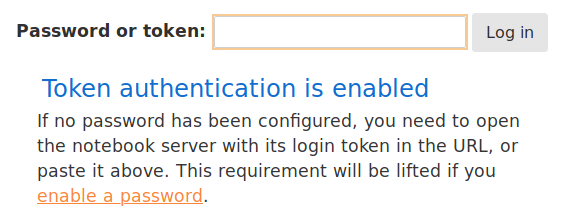
\includegraphics[scale=0.5]{cap01/paginaSenha.png}
	\caption{Jupyter solicitando o Token}
\end{figure}

A senha do token está definida na última linha do Script como "data-science", após informá-la o jupyter está pronto para trabalharmos:
\begin{figure}[H]
	\centering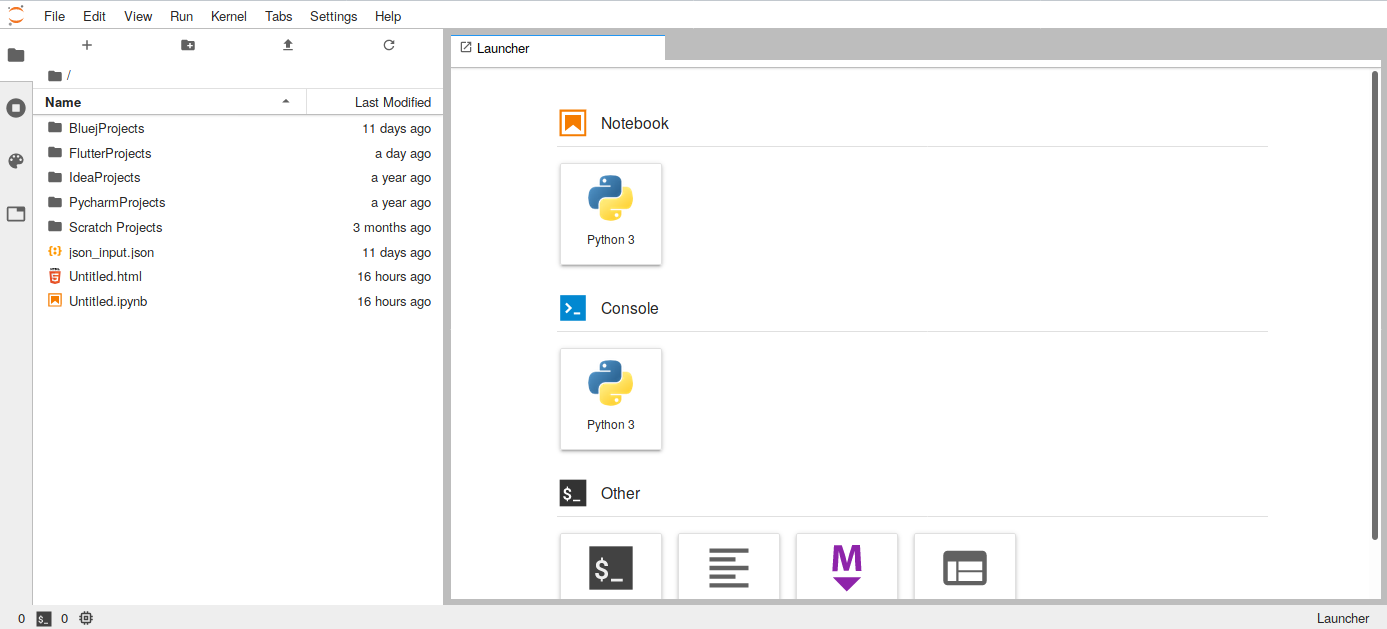
\includegraphics[scale=0.3]{cap01/jupyterLab.png}
	\caption{Jupyter Lab pronto}
\end{figure}

A maior vantagem que agora possuímos um ambiente com o \textbf{Jupyter Lab} completamente controlado incluindo temas e sincronização com o \textbf{Github}. Os próximos comandos são bem mais simples, tais como: \\
{\ttfamily\$ docker stop meu-jupyter} \\
{\ttfamily\$ docker start meu-jupyter}

Respectivamente para encerrar e iniciar o contêiner. Oh não! Agora estou preso, não posso mais fazer atualizações. Devemos entender que os contêineres são \textbf{dinâmicos}. Precisamos instalar o Keras/TensorFlow, acessar o contêiner (com ele já iniciado): \\
{\ttfamily\$ docker exec -it meu-jupyter /bin/bash}

E instalamos normalmente, como se estivesse em uma máquina com o Ubuntu (com os poderes de superusuário): \\
{\ttfamily\# conda install -c conda-forge keras}

Pronto uma vez testado podemos optar por manter só nesse contêiner, ou então modificar o Script para ao criarmos novos contêineres e estes serão criados com essa funcionalidade embutida.

Verificar qual a versão do Python que está a nossa disposição, em uma célula do Notebook digite:
\begin{lstlisting}[]
!python --version
\end{lstlisting}

Ao pressionarmos Ctrl+Enter será mostrada a versão 3.7.7. Agora podemos testar e executar qualquer ferramental sem nos preocuparmos em corromper a máquina. Talvez, no máximo, perdermos um contêiner.
	
\clearpage